\chapter{Hardwarové komponenty} \label{chap:hardware}
V této kapitole je popsán veškerý použitý hardware v projektu senzorického řešení chytré domácnosti. V projektu je využito 5 mikročipů ESP8266, 8 čidel pro měření fyzikálních veličin a jeden počítač Raspberry Pi. 

Měřené fyzikální veličiny lze rozdělit do dvou základních kategorií. Veličiny, které jsou měřeny uvnitř domácnosti v rámci místnosti a veličiny ve venkovním prostředí. Mezi veličiny měřené uvnitř místnosti patří teplota, vlhkost, intenzita osvětlení, stav dveří a oken, barometrický tlak a existence pohybu. Ve venkovním prostředí je měřena teplota. Na \cref{fig:hardware_diagram} je zobrazen použitý hardware v závislosti na měřených veličinách. 

\begin{figure}[H]
  \centering
  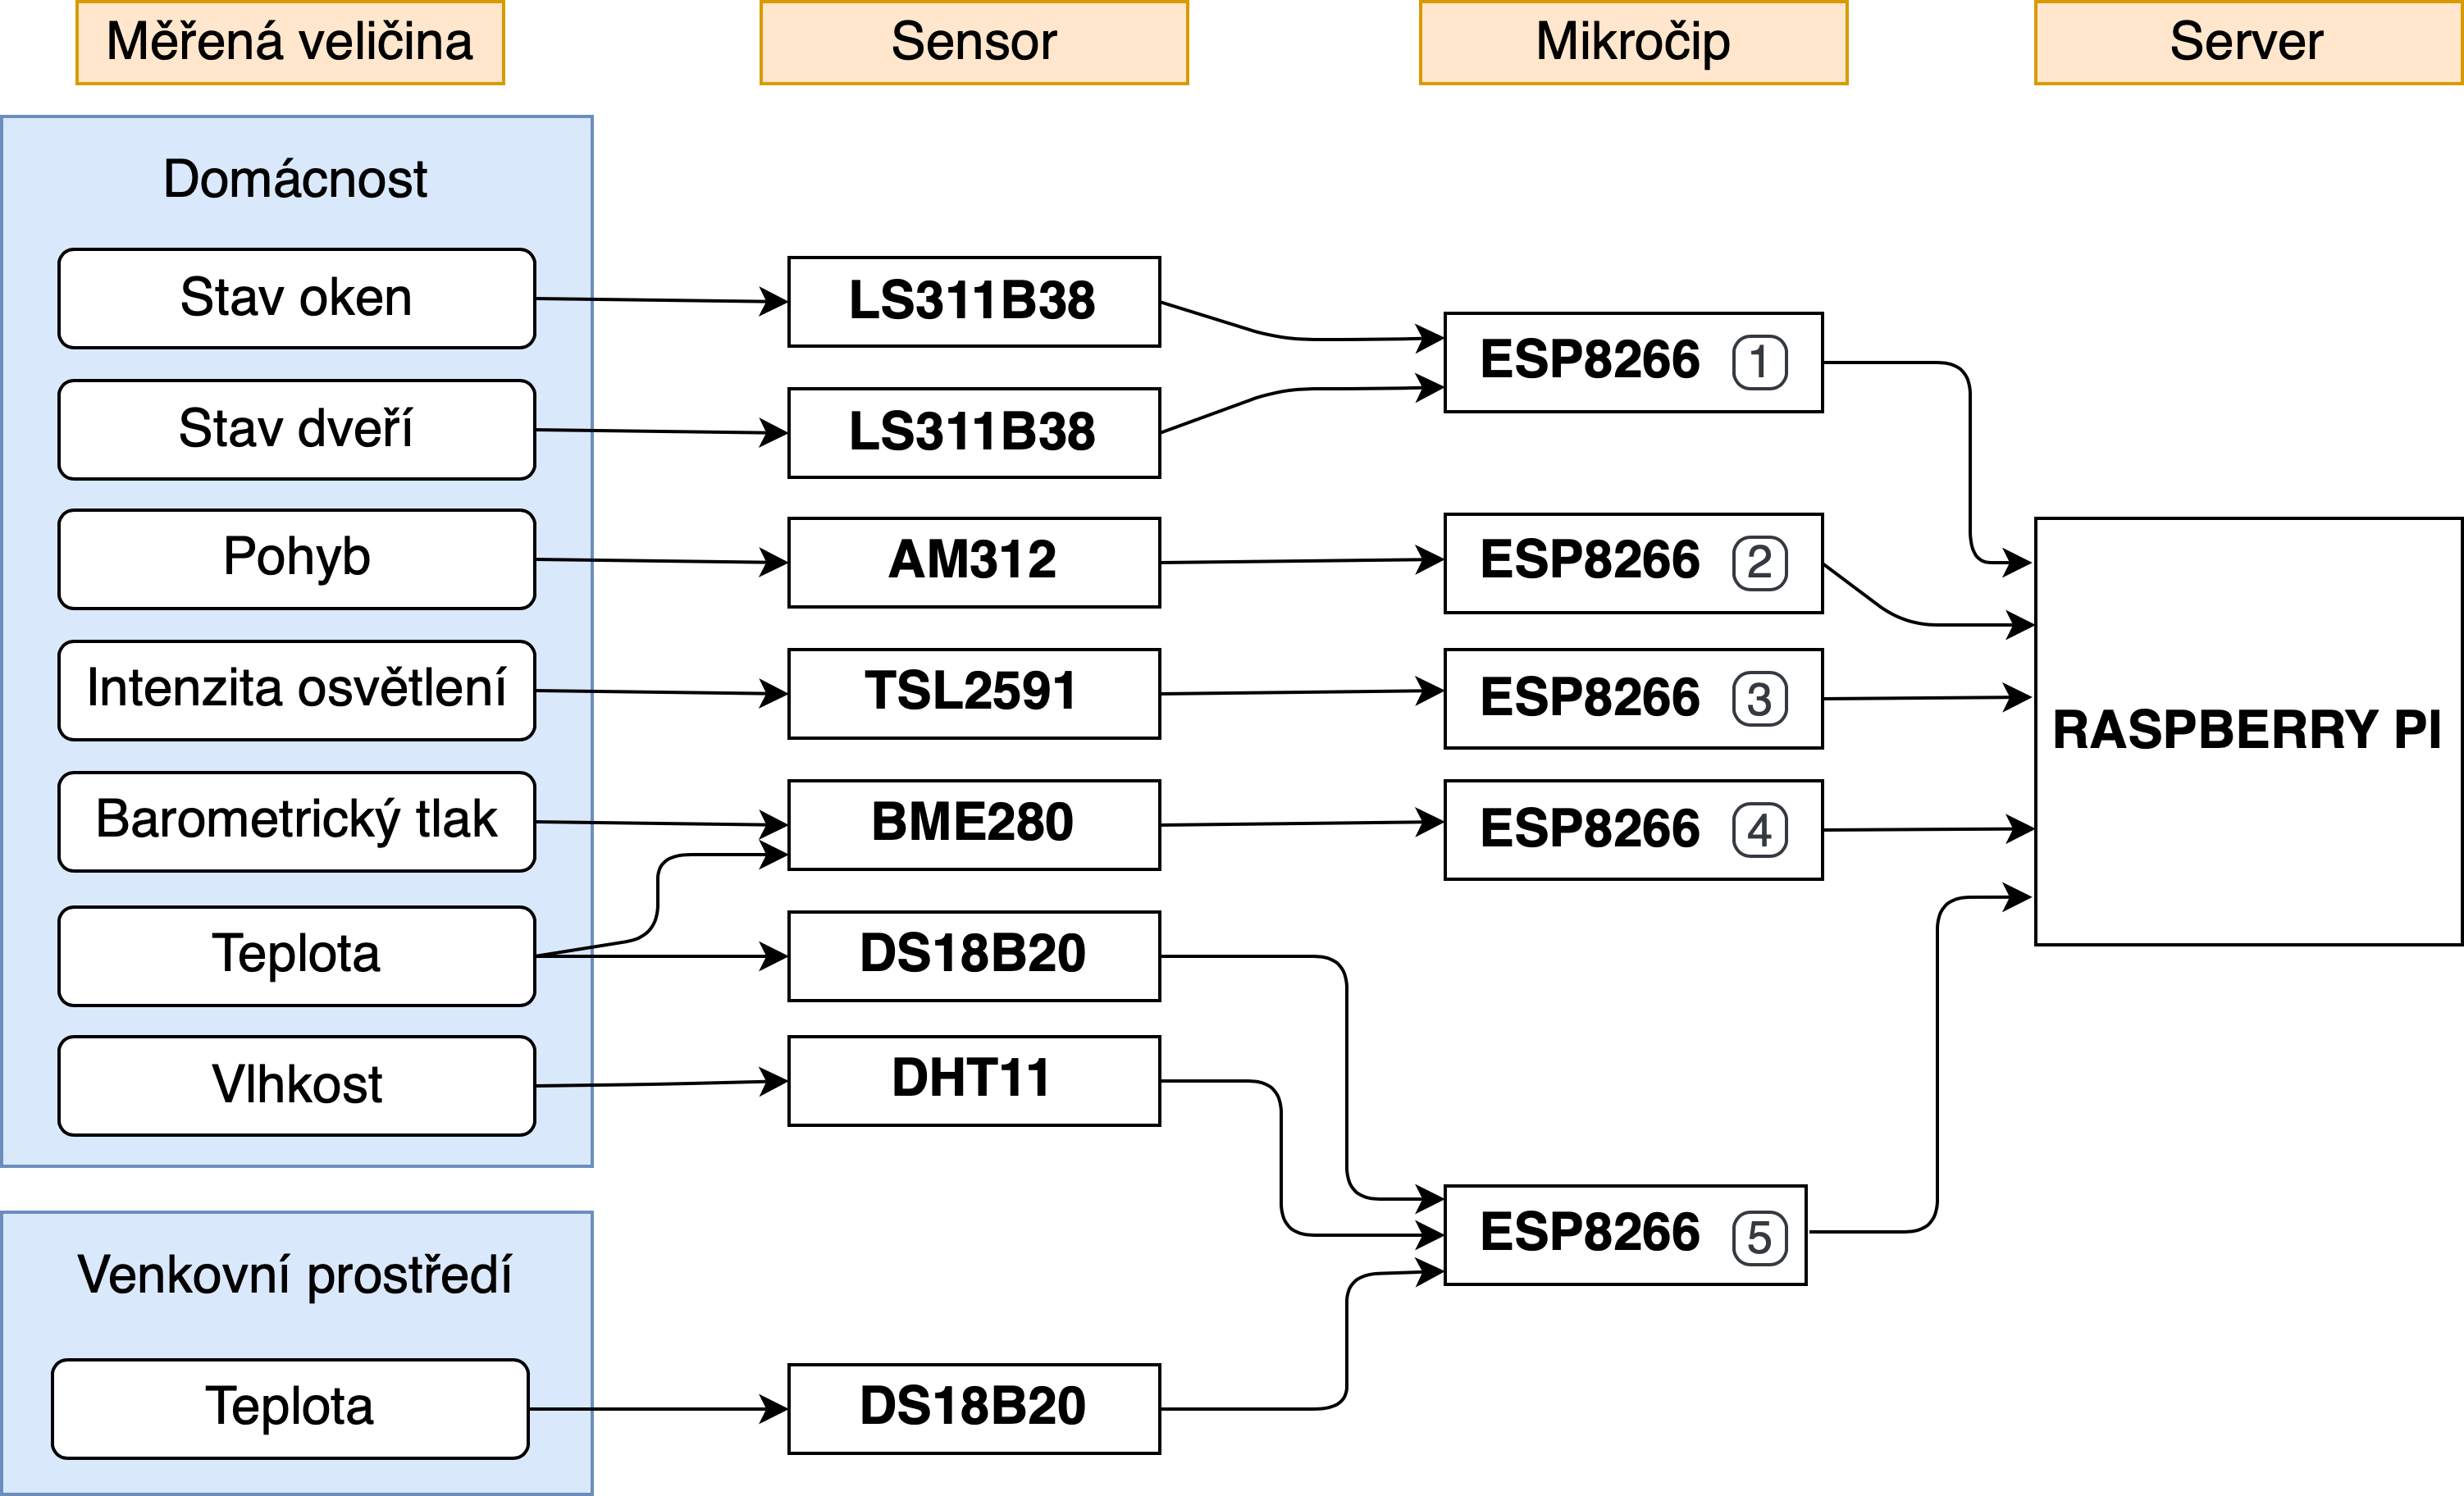
\includegraphics[width=0.9 \textwidth]{hardware_diagram.png}
  \caption{Vztahy mezi použitým hardwarem a měřenými veličinami}
  \label{fig:hardware_diagram}
\end{figure}

Ve snaze o co nejefektivnější využití hardwaru může jeden mikročip číst data z několika čidel. Děje se to hlavně u čidel teploty a vlhkosti a u čidel pro monitorování stavu oken a dveří. U ostatních čidel je zpravidla využit jeden mikročip pro čtení dat z jednoho specifického čidla. Tento přístup byl využit zejména z důvodů specifického fyzického umístění senzoru (např.: pohybový senzor musí být umístěn v rohu místnosti, kde není vhodné současně měřit jiné veličiny) nebo z důvodu výpočetní náročnosti, kdy jeden mikročip zvládne načítat data pouze z jednoho čidla.

\section{Mikročip ESP8266} \label{sec:esp8266}

Základním stavebním prvkem senzorů v této chytré domácnosti je mikročip \textbf{ESP8266}. Existuje celá řada mírně odlišných mikrokontrolérů založených na tomto modulu, v principu se ale jedná o velmi levný mikročip s procesorem o frekvenci 80 Hz, flash pamětí typicky od 512 KiB do 4 MiB, 16 vstupně-výstupních GPIO piny a podporou sběrnic SPI,  I$^2$C a I$^2$S \footnote{https://en.wikipedia.org/wiki/ESP8266}.

\subsection*{Vlastnosti mikročipu}
Hlavní předností toho čipu je podpora Wi-Fi standardu IEEE 802.11 b/g/n. K mikročipu stačí kabelově přivést pouze napájení a veškerá komunikace může probíhat bezdrátově po místní síti. Tím odpadá nutnost předem připravené kabeláže v domě a rozšiřují se možnosti využití i v méně dostupných prostorech. Tento druh mikročipu byl zvolen hlavně kvůli kompatibilitě s celou řadou čidel, podpoře několika programovacích jazyků a v neposlední řadě kvůli široce rozšířené komunitě a dostupnosti nejrůznějších návodů pro DIY projekty.

\subsection*{Vývojové platformy}
Vývojové desky s mikročipem ESP8266 jsou vyráběny v několika provedeních. V projektu chytré domácnosti jsem využil výhradně vývojovou platformu \textbf{NodeMCU} (na \cref{fig:nodemcu}\footnote{Převzato z http://pdacontrolen.com/introduction-platform-iot-cayenne-mydevices-esp8266/}). Tato platforma je přizpůsobena pro pohodlnou komunikaci s mikročipem ESP8266 pomocí sériové linky. Platforma disponuje USB konektorem a vývody GPIO pinů. USB konektor slouží k napájení a zároveň k přenosu dat do paměti mikročipu. Pro zapojení externích komponent a vytváření obvodů lze pohodlně využít breadboard\footnote{Nepájivé kontaktní pole. Komponenta, která umožňuje sestavit prototyp obvodu a je vhodná pro prvotní experimentování.} a propojovací kabely. V fázi vytváření prototypu tedy není nutné pájet.

\begin{figure}[H]
  \centering
  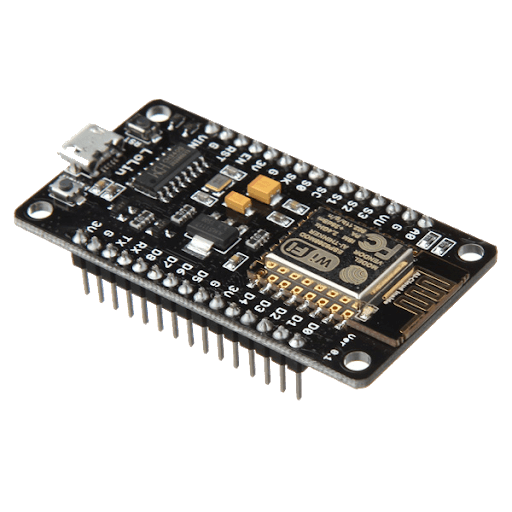
\includegraphics[width=0.4 \textwidth]{nodemcu.png}
  \caption{Vývojová platforma NodeMCU s modulem ESP8266}
  \label{fig:nodemcu}
\end{figure}

\subsection*{Firmware mikročipu}
Po zakoupení vývojové platformy je prvně potřeba nahrát aktuální firmware do flash paměti mikročipu. Před nahráním firmwaru je nutné nainstalovat ovladač pro komunikaci s USB rozhraním na desce. NodeMCU zpravidla vyžaduje ovladač CP2102 (alternativně CH340). Pro nahrání samotného firmwaru do mikročipu jsem zvolil nástroj esptool.py\footnote{https://github.com/espressif/esptool}. Esptool je program postavený na Pythonu, který umí načíst informace o připojeném mikročipu, vymazat flash paměť, nahrát nový firmware a případně zálohovat flash paměť.

\subsection*{Vývojové prostředí}
Tento mikročip není plnohodnotným počítačem ve smyslu jakéhokoliv uživatelského rozhraní. Veškerá komunikace s čipem probíhá po USB rozhraní a je založena na principu nahrání skriptů do paměti čipu a následném restartování pro spuštění programu. Jakákoliv změna kódu znamená vymazání původního skriptu z paměti čipu a následném nahrání nového skriptu. Tato skutečnost mírně ztěžuje ladění kódu a odchytávání chyb, ale samotný skript pro mikrokontrolér nebývá příliš dlouhý a k ladění kódu lze efektivně využít příkazovou řádku. Pro ukládání skriptů do mikročipu je potřeba vhodný nástroj pro přístup do adresářové části paměti na čipu. Jedním z těchto nástrojů je Mpfshell\footnote{https://github.com/wendlers/mpfshell}. Mpfshell je balíček postavený na Pythonu, který umožňuje editaci souborů uložených v paměti (nahrávání, mazání, vytváření složek apod.) a zpřístupňuje příkazovou řádku na mikročipu. Právě příkazová řádka je zásadní pro rychlé spuštění kódu a odladění chyb, je možné v ní přímo psát části kódu nebo spouštět jednotlivé skripty bez nutnosti restartu.

\subsection*{Programování mikročipu}
Samotné ESP8266 může být programováno v několika jazycích, předně v Arduino IDE, MicroPythonu nebo LUA. V tomto projektu jsou všechny mikrokontroléry programovány v jazyce MicroPython. V rámci sjednocení programovacích jazyků v celém projektu jsem vybral MicroPython právě z důvodu univerzálnosti. MicroPython vychází z Pythonu 3 a je přímo přizpůsoben pro programování mikrokontrolérů. Další části projektu (například backend webové vizualizace nebo klasifikátor dat) jsou postaveny na Pythonu 3, proto se MicroPython v rámci zachování jednotné struktury jevil jako logická volba. Nespornou výhodou tohoto jazyku je velká podpora v rámci komunity a množství návodů a knihoven pro komunikaci s jednotlivými čidly. 

\subsection*{Postup fyzické realizace čidel}
Prvním krokem při návrhu chytrých čidel je stanovení fyzikálních veličin, které chceme sledovat a otestovat spolehlivost čidel pro měření těchto veličin. Po vybrání konkrétních senzorů následuje sestrojení prototypu - zapojení obvodu na breadboardu. Po vytvoření funkčního obvodu může začít experimentování a ladění kódu pro načítání dat z čidla. Po úspěšném naprogramování komunikace s čidlem jsem přešel k vytvoření pevného fyzického obvodu napájením jednotlivých součástí na plošný spoj. Tento plošný spoj má nespornou výhodu ve své životnosti a odolnosti, na rozdíl od obvodu na breadboardu, kde se kabely mohou vlivem neopatrnosti vypojovat. Ke každému senzoru jsem přidal červenou externí led diodu pro indikaci různých změn a stavů. Uživatel v podstatě nemá žádný jiný způsob vizuální kontroly funkčnosti senzoru. Led diodu využívám jako signalizaci při úspěšném připojení k Wi-Fi a jako signalizaci odeslání zprávy. Vždy, když senzor odešle zprávu, dioda jednou blikne. 

\subsection*{Architektura kódu na mikročipu}
Kód v MicroPythonu pro mikrokontrolér ESP8266 sestává z několik částí. Primárně se jedná o soubor \textit{boot.py} a \textit{main.py}. Soubor \textit{boot.py} se po zapnutí mikrokontroléru spustí vždy jako první nezávisle na jakémkoliv dalším souboru. V tomto skriptu dochází k připojení k místní Wi-Fi síti. Po úspěšném připojení k síti senzor čtyřikrát zabliká interní led a následně i externí led diodou pro vizuální kontrolu. Druhým skriptem, který naběhne ihned po \textit{boot.py} je \textit{main.py}. Toto pořadí a dané dva skripty jsou pevně stanovené programovacím jazykem nezávisle na implementaci dalších skriptů.
V senzorech pro chytrou domácnost se uplatňují 2 základní přístupy odesílání dat na server. První je založen na odeslání zprávy na základě vzniku události a druhý přístup odesílá zprávy pravidelně s předem zvolenou periodou odesílání. V obou případech se po zapnutí senzoru mikročip nejprve připojí k Wi-Fi a problikne led dioadami. Tento proces proběhne jednorázově a pak senzor přejde do stavu, kdy je připraven načítat data ze senzorů a publikovat zprávy.

 \subsection*{Odesílání zpráv na základě vzniku události}
Odesílání zpráv ze senzoru na server na základě vzniku události používá senzor pro detekci pohybu v místnosti a senzor pro monitorování stavu oken a dveří. Tento přístup je popsán v diagramu na \cref{fig:esp_event_based_diagram}. V nekonečném cyklu, do kterého se senzor dostane po připojení k internetu, se prvně sesynchronizuje čas se světovým časem pomocí protokolu NTP\footnote{\textbf{N}etwork \textbf{T}ime \textbf{P}rotocol - protokol pro synchronizaci času počítače po internetu}. Po synchronizaci senzor čeká dokud se neobjeví událost, kterou má zaznamenat. Touto událostí je například otevření či zavření okna nebo dveří a nebo pohyb člověka v místnosti. V této části kódu tedy čidlo setrvává naprostou většinu času. V momentě, kdy událost nastane, čidlo problikne externí led diodou (v případě pohybového čidla se pro indikaci zapne ještě externí bzučák) a přejde do fáze vytváření zprávy. Po vytvoření struktury zprávy, která sestává z několika atributů (více v \cref{sec:protocol_mqtt}), se senzor připojí k MQTT brokeru a odešle zprávu. Po odeslání zprávy se uspí na 3 vteřiny a celý cyklus se opakuje. Uspání je v programu spíše jako preventivní opatření, aby se kód nežádaným způsobem někde nazacyklil. V případě pohybového senzoru je krátké uspání vhodné také pro to, aby čidlo neposílalo zbytečně moc zpráv, když se v místnosti vyskytuje pohyb. Šetří se tím vytíženost sítě a pro účel detekce pohybuje není nutné odesílat informaci několikrát za vteřinu.

\textcolor{red}{více v sec 3.1 přeložit do češtiny}

\begin{figure}[H]
  \centering
  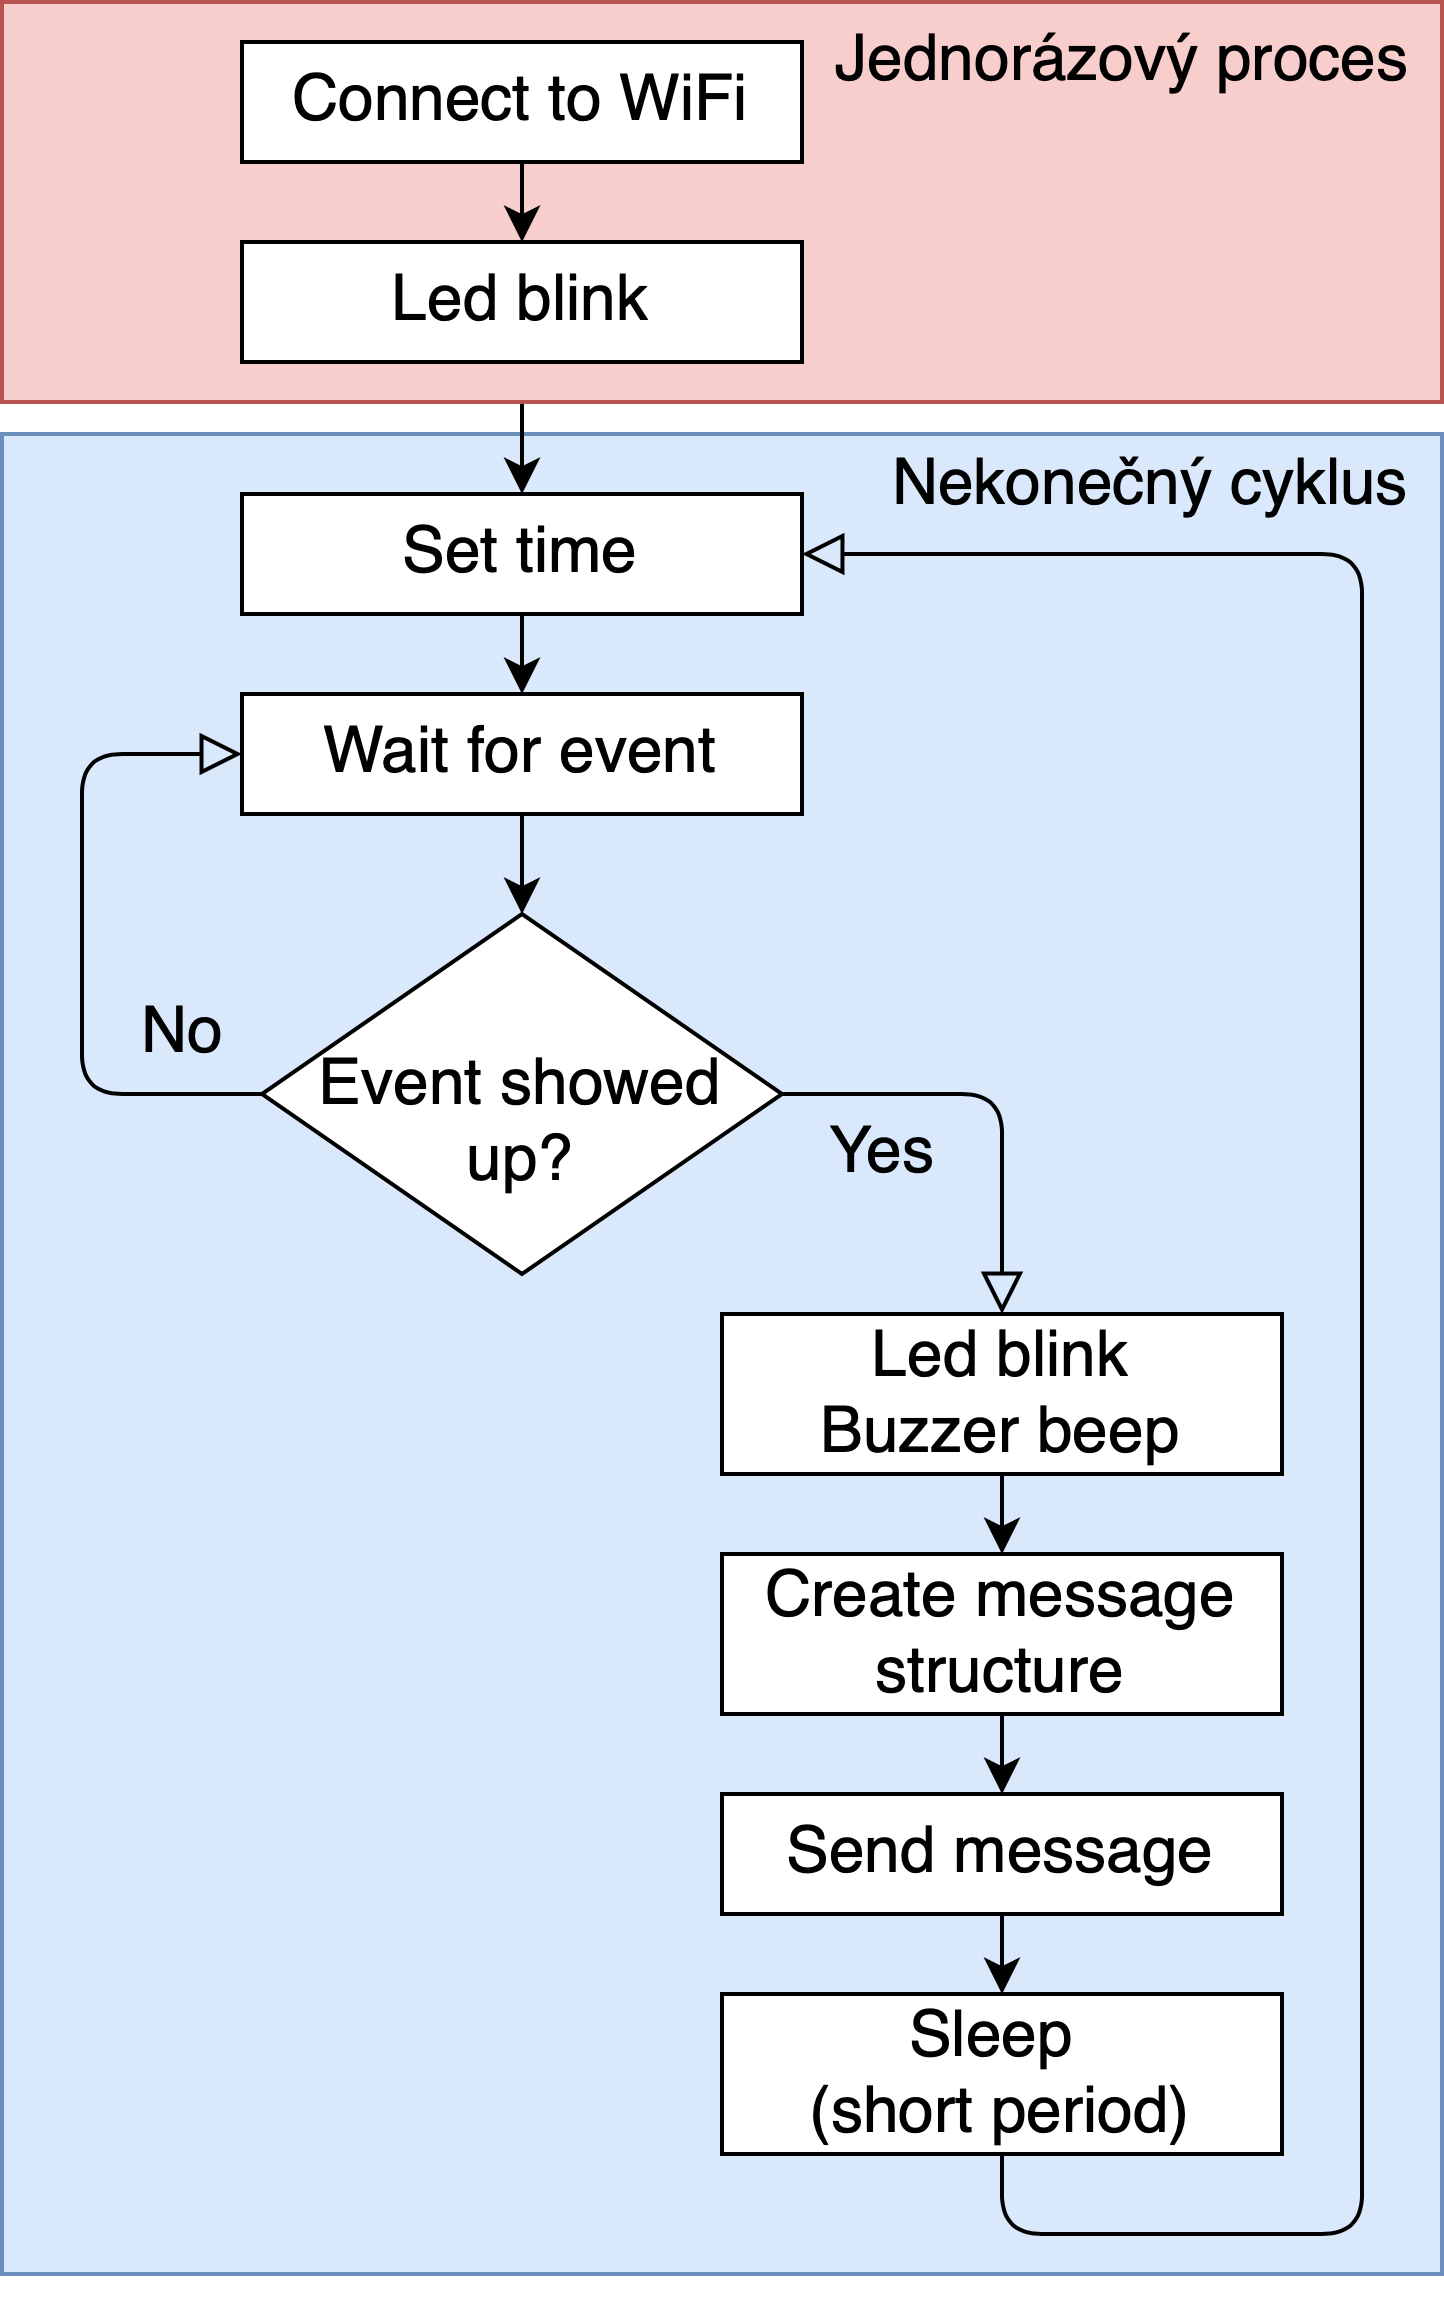
\includegraphics[width=0.5 \textwidth]{esp_event_based_diagram.png}
  \caption{Diagram odesílání zpráv na základě vzniku události}
  \label{fig:esp_event_based_diagram}
\end{figure} 
 
 \subsection*{Periodické odesílání zpráv}
Pravidelné odesílání zpráv s předem danou frekvencí odesílání používají všechny ostatní senzory, které měří veličiny, u kterých je vhodné měření po určité době opakovat. Jde o čidla vnitřní a venkovní teploty, vlhkosti, intenzity osvětlení a barometrického tlaku. U těchto senzorů je vhodné měření fyzikálních veličin opakovat za účelem získání dostatečného množství dat pro následné trénování modelů a klasifikaci. 

\begin{figure}[H]
  \centering
  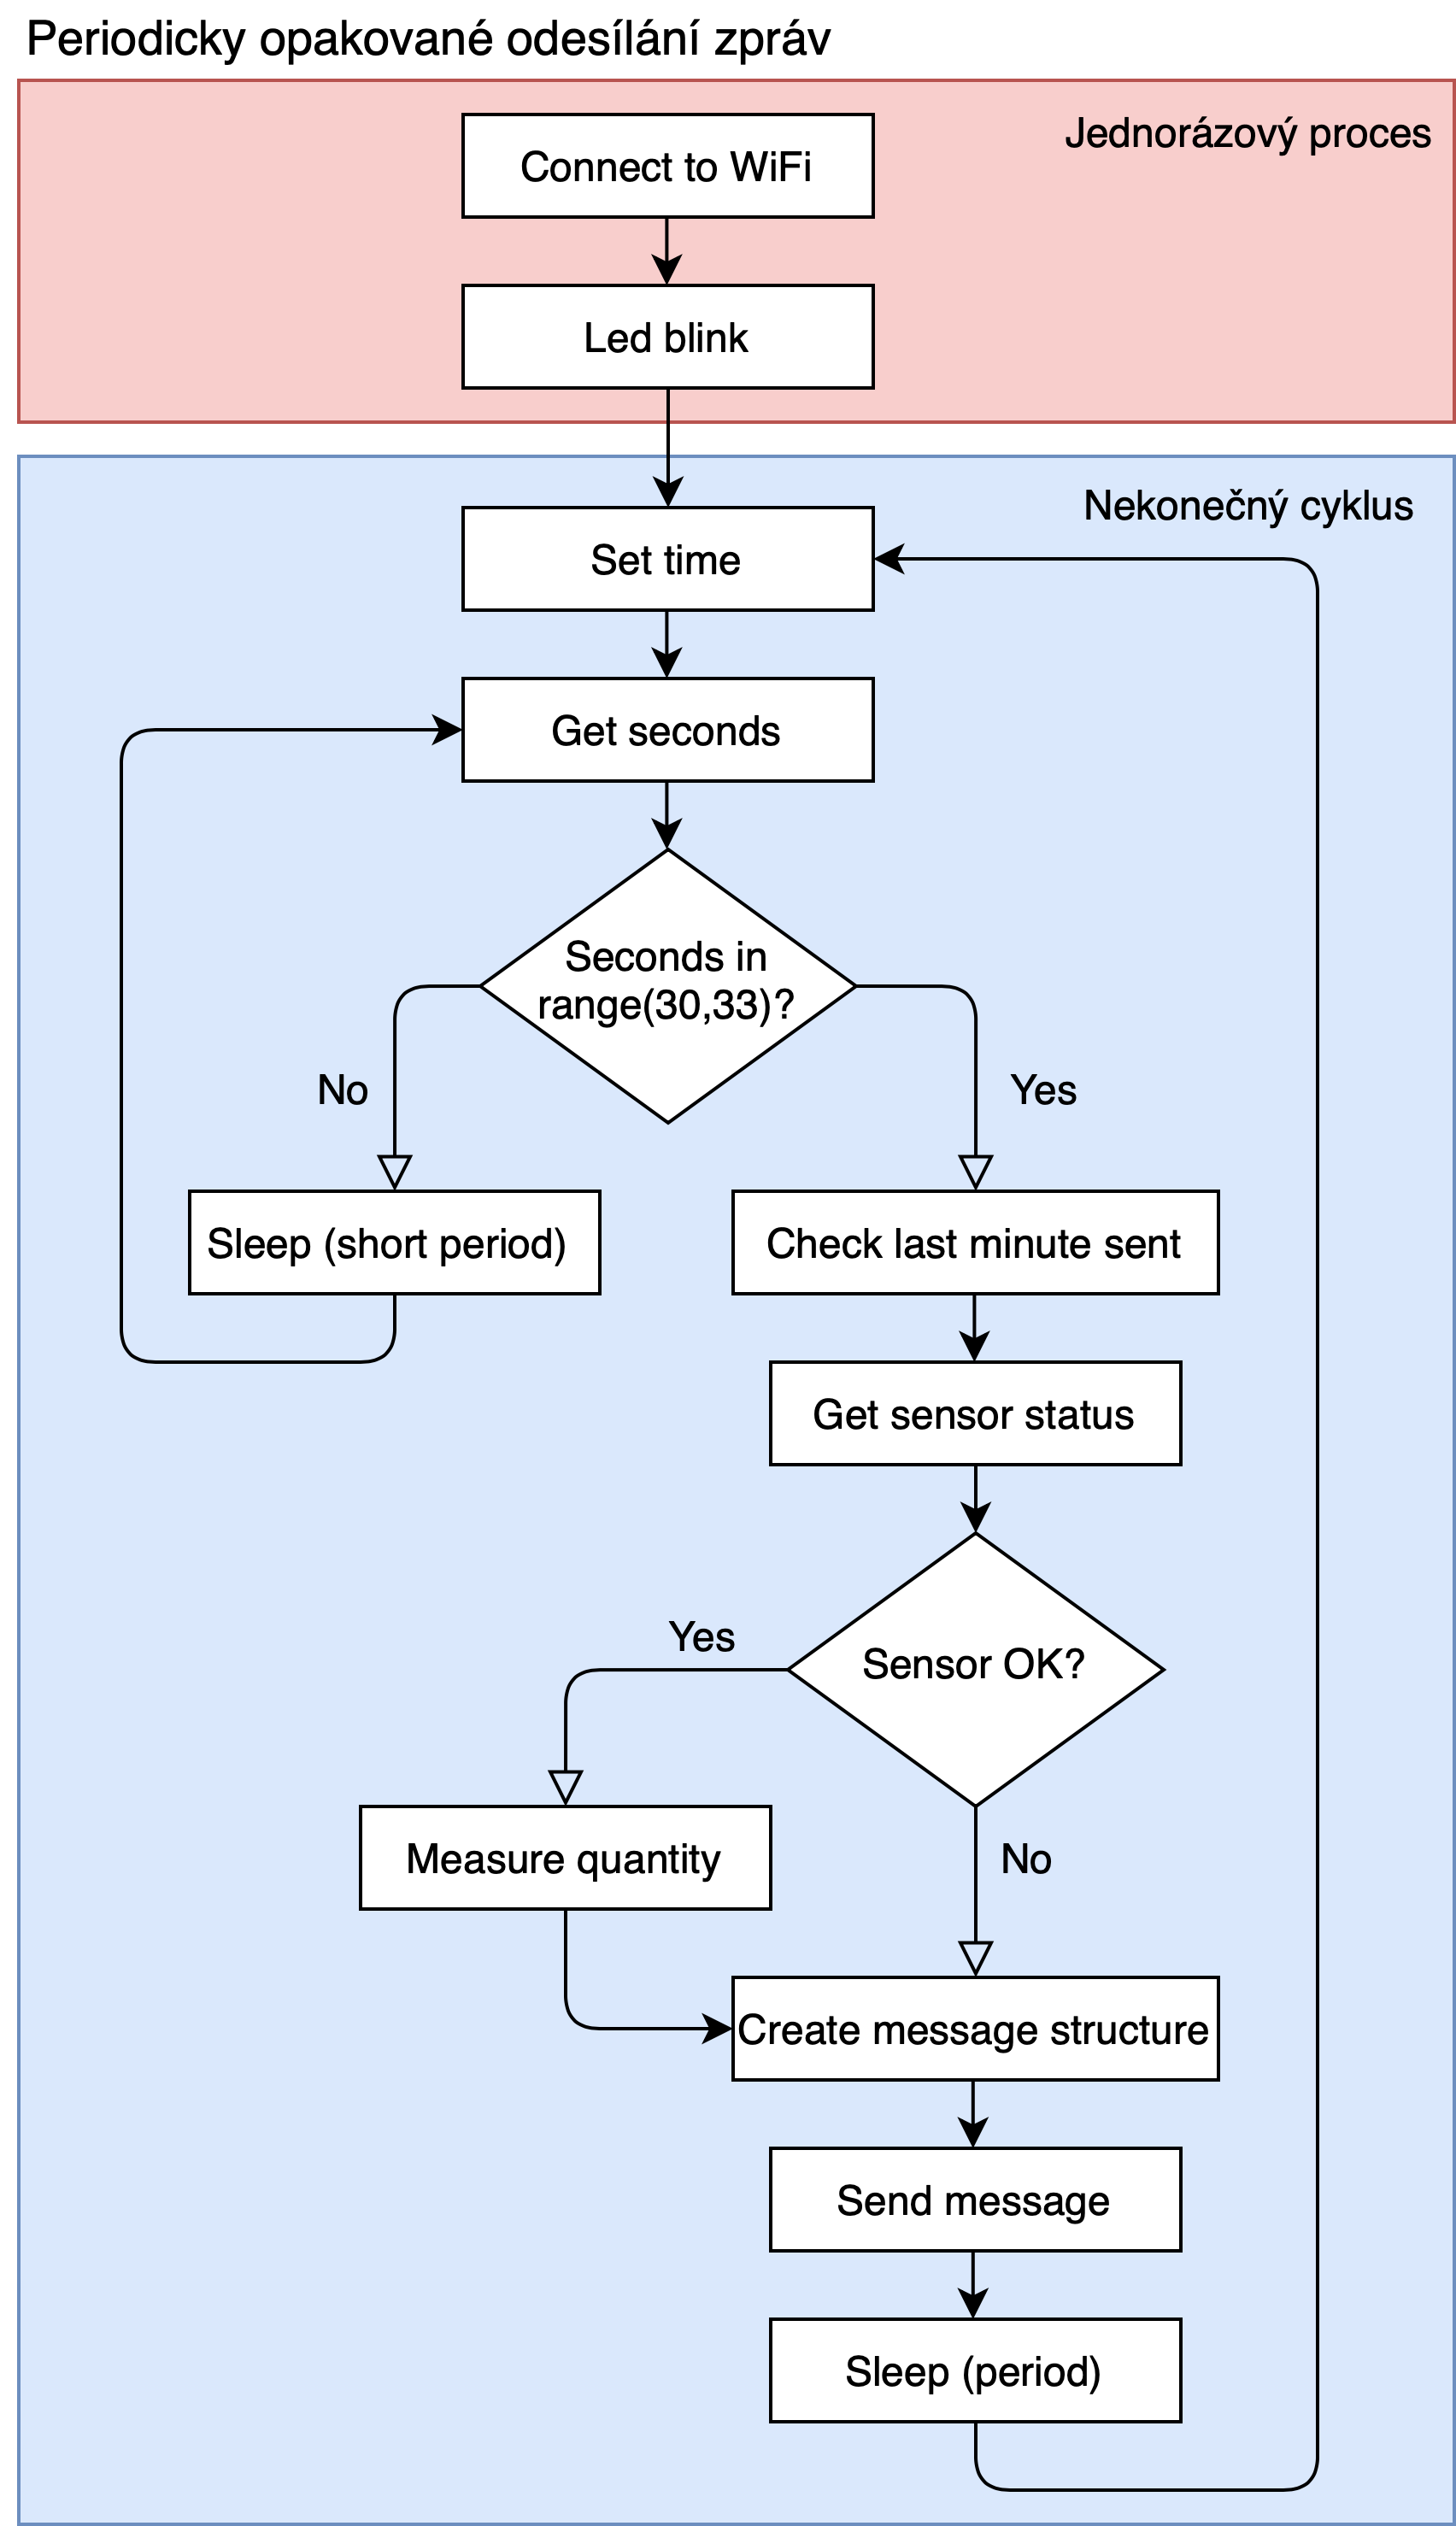
\includegraphics[width=0.5 \textwidth]{esp_periodical_diagram.png}
  \caption{Diagram periodicky opakovaného odesílání zpráv}
  \label{fig:hardware_components:LABEL}
\end{figure}


Vytvoření designu a vytvoření pevného obvodu - ESP + čidlo na PCB desce \\
Popis logiky komunikace mezi ESP, jednotlivými čidly a odesíláním zpráv (prvně připojit k wifi -> načíst hodnotu měřené veličiny -> v případě, že hodnota OK -> odeslat zprávu na broker -> uspat se) \\
Naprogramování logiky ESP - dva použité principy (periodické odesílání zpráv nebo odesílání zpráv založené na události) \\
Objektově orientovaná struktura kódu na ESP - boot.py, main.py, config.py, mqttclient.py, skript pro načítání dat z konkrétního senzoru (důraz kladen na objektové programování - přehlednost kódu, snadné změny, konfigurační soubor pro nastavení vstupních parametrů, univerzální kód pro všechna esp, snadná rozšiřitelnost kódu do budoucna, snadná implementace dalších senzorů, ...) \\



 \subsection*{Detail architektury kódu na mikročipu}
Architektura kódu všech senzorů sestává ze stejného základu. Při návrhu programu pro mikročipy byl kladen důraz na objektovou strukturu programování a co nejuniverzálnější využití. Proto je základ programu pro všechny senzory stejný a liší se jen komunikací s konkrétním čidlem. Tímto přístupem se podařilo sjednotit verze kódu ve všech senzorech a hlavně umožnit rychlé přidání dalších senzorů v budoucnu. Pokud bych do chytré domácnosti chtěl přidat další senzor, který bude měřit jinou fyzikální veličinu, nemusím programovat celou logiku senzoru znovu nebo složitě vytrhávat části jinde použitého kódu, ale použiji stávající program, který pouze doplním o implementaci komunikace s konkrétním čidlem. 

\begin{figure}[H]
  \centering
  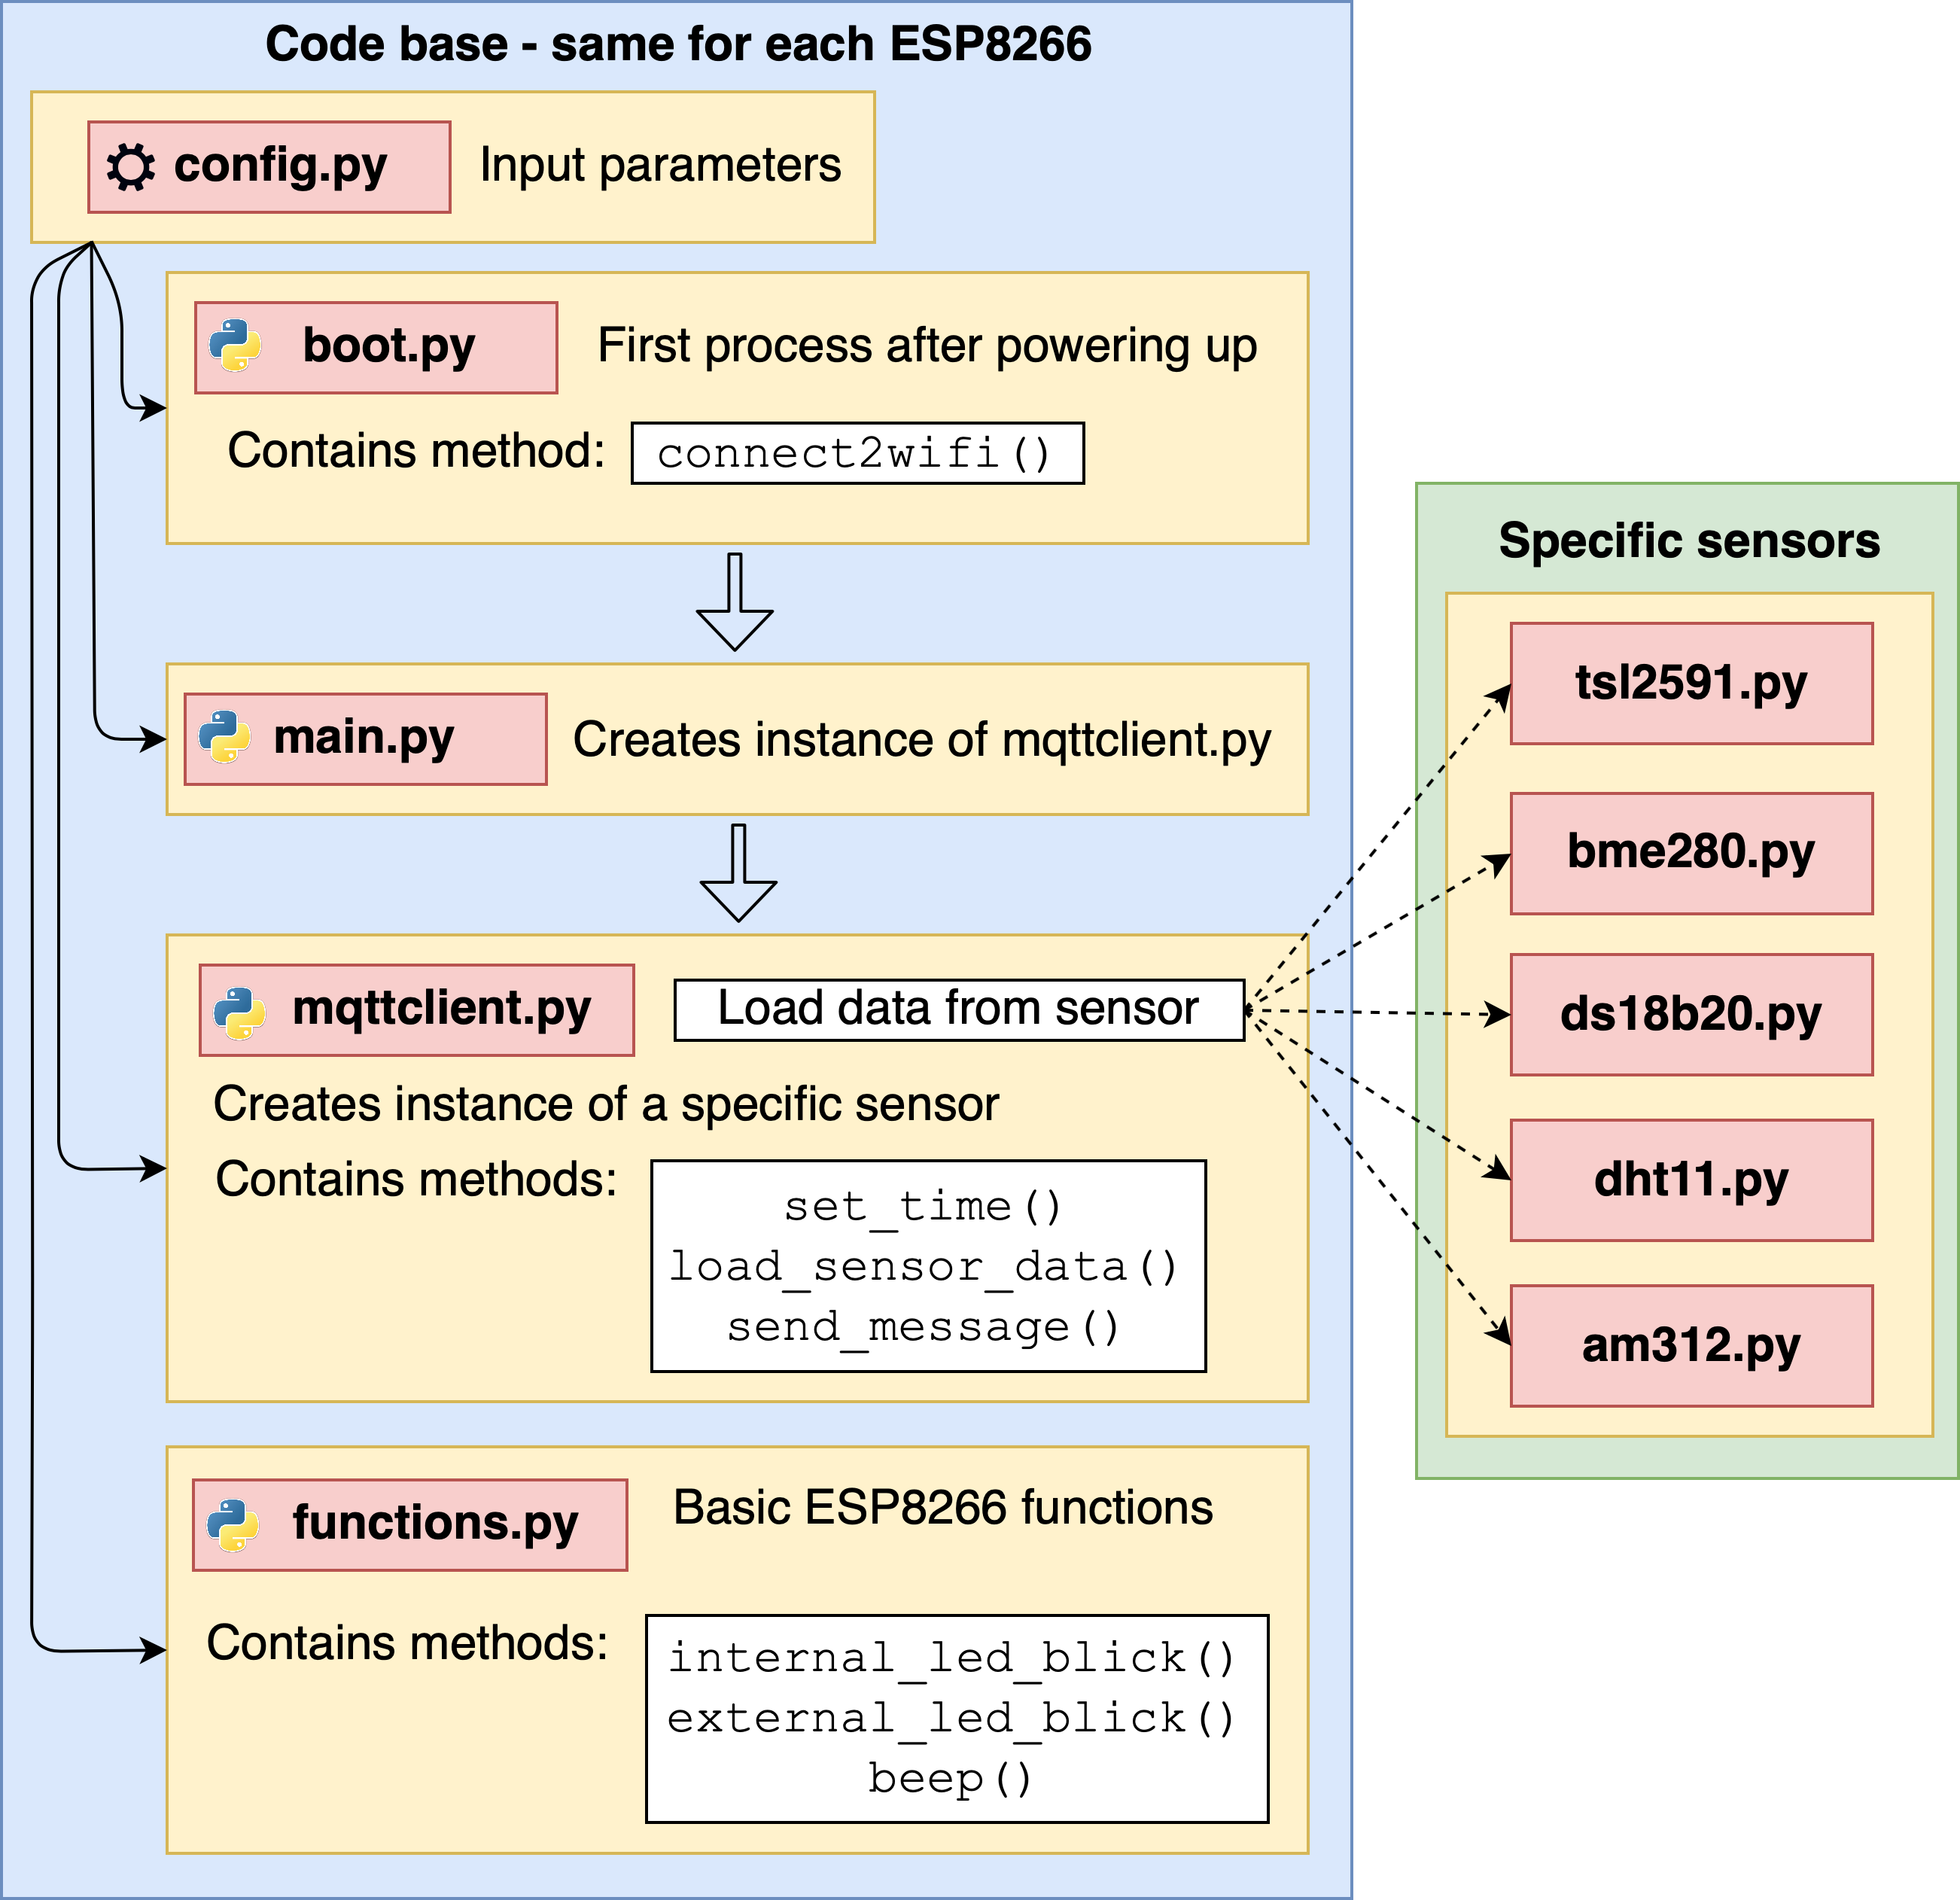
\includegraphics[width=0.9 \textwidth]{esp_code_architecture.png}
  \caption{Diagram architektury kódu na microchipu ESP8266}
  \label{fig:hardware_components:LABEL}
\end{figure}

\section{Senzory} \label{sec:example_xor}

V projektu chytré domácnosti bylo použito celkem 7 senzorů pro měření fyzikálních veličin ... \\
Které veličiny měřeny (využití naměřených hodnot, smysl měřených veličin, ...) \\
Proč vybrány tyto konkrétní senzory \\

\subsection{Teplotní čidlo DS18B20}

esp-temphumid \\
Senzor pro měření teploty \\
Základní informace o senzoru - rozsah měření, přesnost, napájení, způsob komunikace, životnost, spolehlivost, ... \\
Více variant - vnitřní, venkovní \\
Obvod zapojení - esp, senzor, rezistor, napájení obvodu na PCB desku, umístění v místnosti \\
Zprovoznění komunikace s teplotními čidlem ds18b20 (room a outside) \\
Schéma zapojení senzoru, esp8266 a dalších periferií (led světlo, bzučák, ...) \\
Fotka reálného zkonstruovaného čidla \\

Senzor DS18B20 je jedním z nejdostupnějších senzorů použitých v projektu chytré domácnosti ...

\begin{figure}[H]
  \centering
  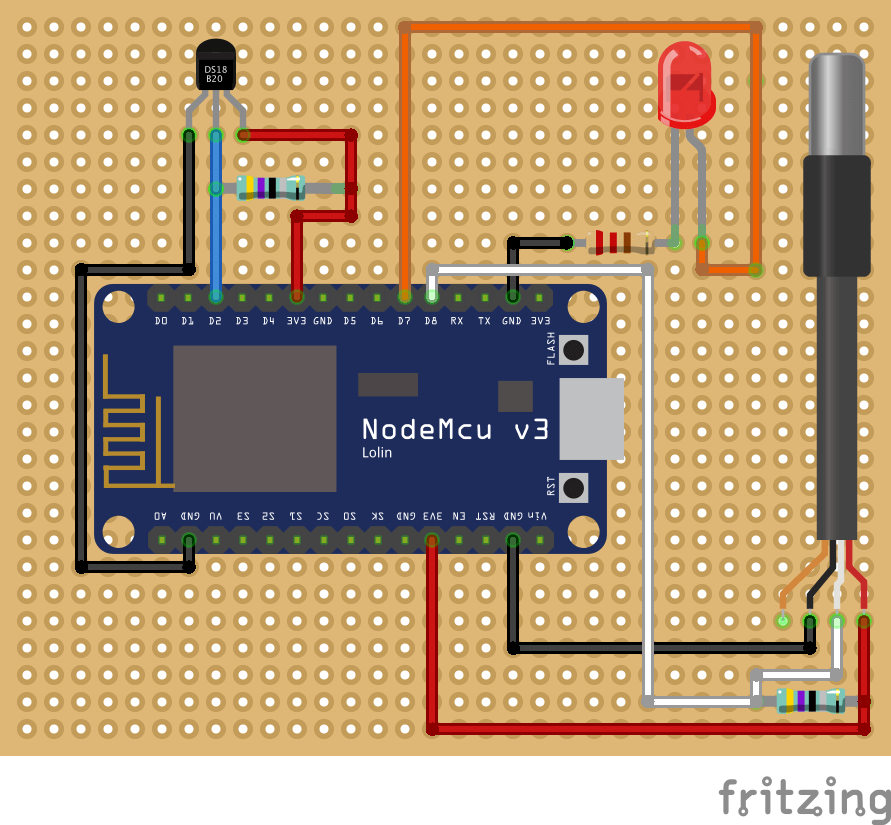
\includegraphics[width=0.7 \textwidth]{ds18b20.png}
  \caption{POPIS}
  \label{fig:hardware_components:LABEL}
\end{figure}

\subsection{Vlhkoměr DHT11}

esp-temphumid \\
Senzor pro měření teploty a  vlhkosti v místnosti \\
Základní informace o senzoru - rozsah měření, přesnost, napájení, způsob komunikace, životnost, spolehlivost, ... \\
Využití měřených veličin (používáme pouze naměřenou vlhkost, protože teplota má oproti ds18b20 nebo bme280 menší přesnost, ...) \\
Obvod zapojení - esp, senzor, rezistor, napájení obvodu na PCB desku, umístění v místnosti \\
Zprovoznění komunikace s vlhkostním čidlem dht11\\
Schéma zapojení senzoru, esp8266 a dalších periferií (led světlo, bzučák, ...) \\
Fotka reálného zkonstruovaného čidla \\

Senzor DHT11 je ...

\begin{figure}[H]
  \centering
  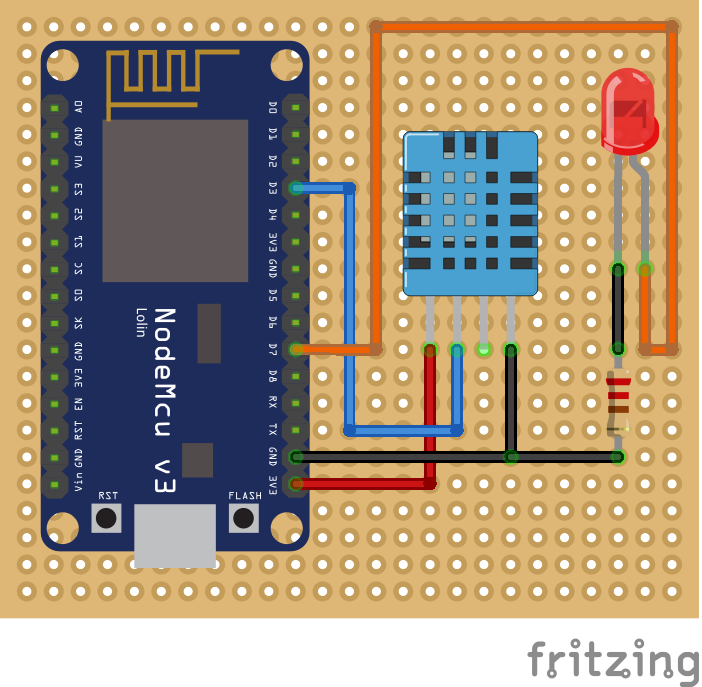
\includegraphics[width=0.7 \textwidth]{dht11.png}
  \caption{POPIS}
  \label{fig:hardware_components:LABEL}
\end{figure}

\subsection{Čidlo intenzity osvětlení TSL2591}

esp-lux \\
Čidlo pro měření intenzity osvětlení \\
Základní informace o senzoru - rozsah měření, přesnost, napájení, způsob komunikace, životnost, spolehlivost, ... \\
Obvod zapojení - esp, senzor, rezistor, napájení obvodu na PCB desku, umístění v místnosti \\
Zprovoznění komunikace se senzorem tsl2591 \\
Schéma zapojení senzoru, esp8266 a dalších periferií (led světlo, bzučák, ...) \\
Fotka reálného zkonstruovaného čidla \\

Senzor TSL2591 je ...

\begin{figure}[H]
  \centering
  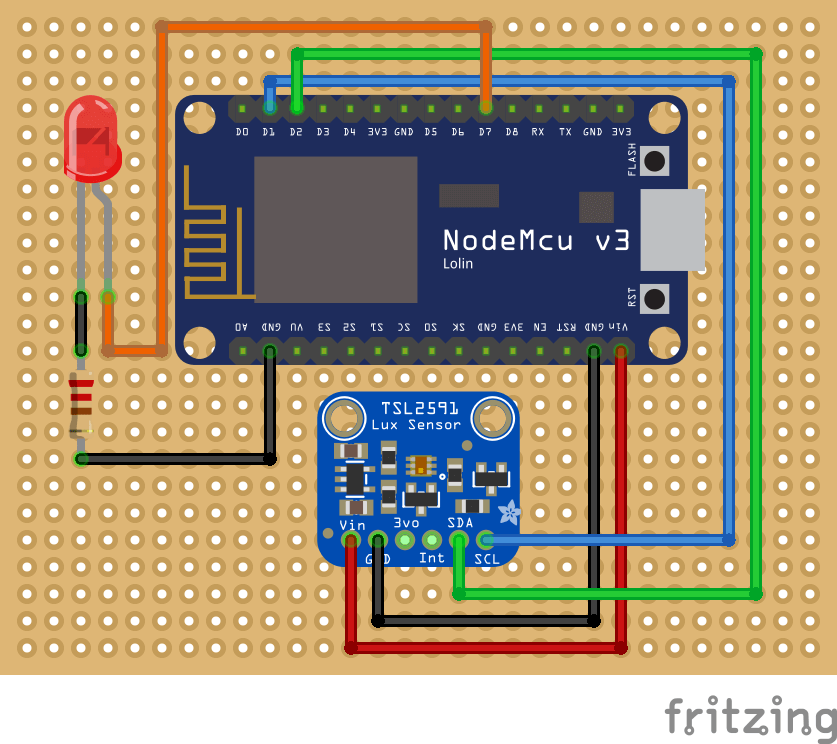
\includegraphics[width=0.7 \textwidth]{tsl2591.png}
  \caption{POPIS}
  \label{fig:hardware_components:LABEL}
\end{figure}

\subsection{Čidlo barometrického tlaku a teploty BME280}

esp-pressure \\
Čidlo pro monitorování vnitřní teploty a barometrického tlaku \\
Základní informace o senzoru - rozsah měření, přesnost, napájení, způsob komunikace, životnost, spolehlivost, ... \\
Obvod zapojení - esp, senzor, rezistor, napájení obvodu na PCB desku, umístění v místnosti, alternativní senzory \\
Zprovoznění komunikace s čidlem bme280 \\
Schéma zapojení senzoru, esp8266 a dalších periferií (led světlo, bzučák, ...) \\
Fotka reálného zkonstruovaného čidla \\

Senzor BME280 je ...

\begin{figure}[H]
  \centering
  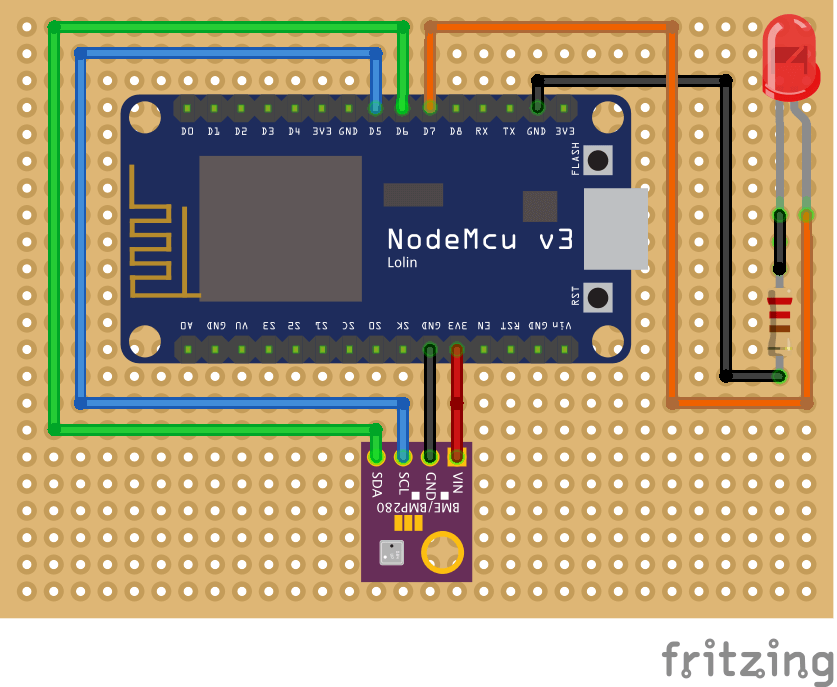
\includegraphics[width=0.7 \textwidth]{bme280.png}
  \caption{POPIS}
  \label{fig:hardware_components:LABEL}
\end{figure}

\subsection{Pohybové čidlo AM312}

esp-pir \\
Čidlo pro monitorování pohybu v místnosti \\
Základní informace o senzoru - rozsah měření, přesnost, napájení, způsob komunikace, životnost, spolehlivost, ... \\
Obvod zapojení - esp, senzor, rezistor, napájení obvodu na PCB desku, umístění v místnosti, alternativní senzory - potíže s čidlem hc-sr501\\
Zprovoznění komunikace se senzorem am312 \\
Schéma zapojení senzoru, esp8266 a dalších periferií (led světlo, bzučák, ...) \\
Fotka reálného zkonstruovaného čidla \\

Senzor AM312 je ...

\begin{figure}[H]
  \centering
  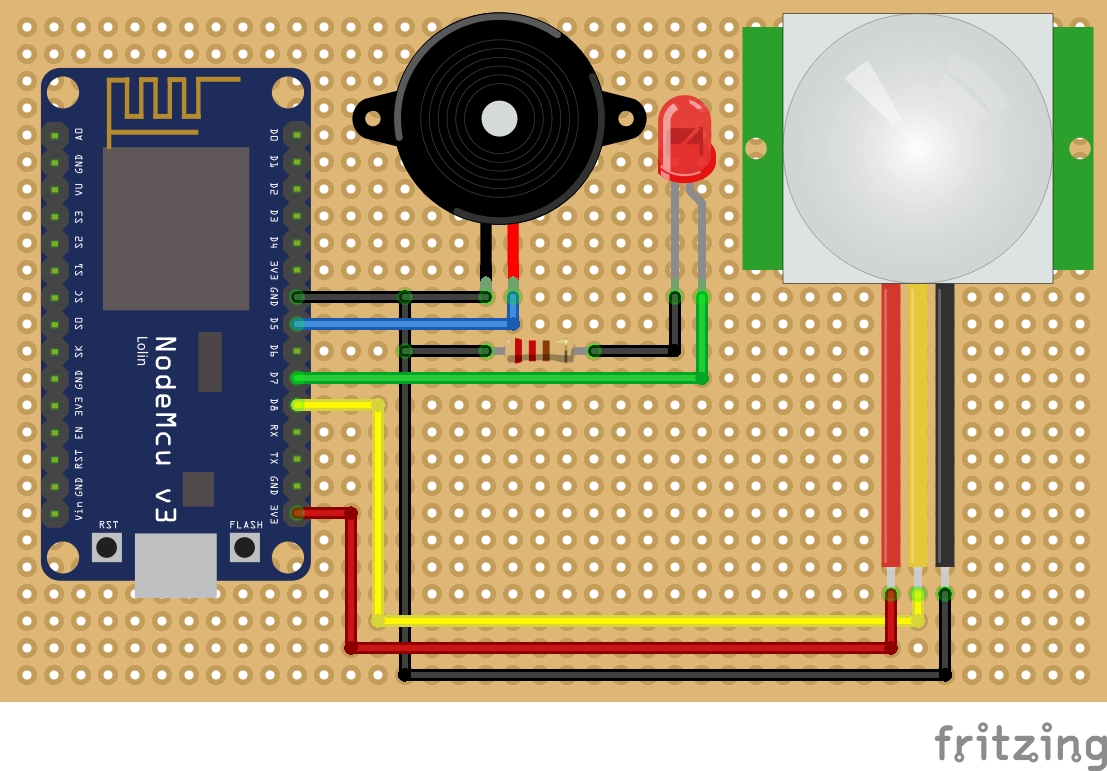
\includegraphics[width=0.7 \textwidth]{am312.png}
  \caption{POPIS}
  \label{fig:hardware_components:LABEL}
\end{figure}

\subsection{Magnetické čidlo LS311B38}

esp-magnet \\
Čidlo pro monitorování stavu dveří a oken \\
Základní informace o senzoru - rozsah měření, přesnost, napájení, způsob komunikace, životnost, spolehlivost, ... \\
Obvod zapojení - esp, senzor, rezistor, napájení obvodu na PCB desku, umístění v místnosti \\
Zprovoznění komunikace s magnetickým senzorem ls311b38 \\
Schéma zapojení senzoru, esp8266 a dalších periferií (led světlo, bzučák, ...) \\
Fotka reálného zkonstruovaného čidla \\

Senzor LS311B38 je ...

\begin{figure}[H]
  \centering
  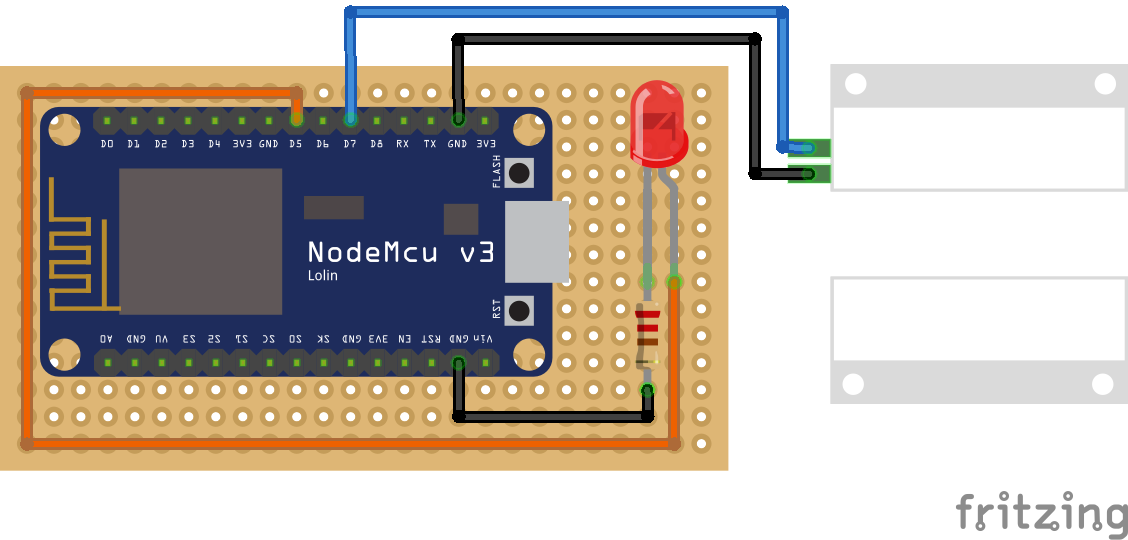
\includegraphics[width=0.7 \textwidth]{ls311b38.png}
  \caption{POPIS}
  \label{fig:hardware_components:LABEL}
\end{figure}

\section{Raspberry Pi} \label{sec:example_xor}

Co je to Raspberry Pi \\
Výhody, nevýhody oproti klasickému pc (výpočetní výkon, spotřeba proudu, ... ) \\
Využití v projektu chytré domácnosti - MQTT broker, databázový server, webserver, klasifikace příchozích zpráv \\
Výhody, nevýhody univerzálního použití Raspberry Pi pro několik účelů, ... \\